
%%%%%%%%%%%%%%%%%%%%%%%%%%%%%%%%%%%%%%%%%%%%%%%%%%%%%%%%%%%%%%%%%%%%%%%%%%%%%%
%  ************************** AVISO IMPORTANTE **************************    %
%                                                                            %
% Éste es un documento de ayuda para los autores que deseen enviar           %
% trabajos para su consideración en el Boletín de la Asociación Argentina    %
% de Astronomía.                                                             %
%                                                                            %
% Los comentarios en este archivo contienen instrucciones sobre el formato   %
% obligatorio del mismo, que complementan los instructivos web y PDF.        %
% Por favor léalos.                                                          %
%                                                                            %
%  -No borre los comentarios en este archivo.                                %
%  -No puede usarse \newcommand o definiciones personalizadas.               %
%  -SiGMa no acepta artículos con errores de compilación. Antes de enviarlo  %
%   asegúrese que los cuatro pasos de compilación (pdflatex/bibtex/pdflatex/ %
%   pdflatex) no arrojan errores en su terminal. Esta es la causa más        %
%   frecuente de errores de envío. Los mensajes de "warning" en cambio son   %
%   en principio ignorados por SiGMa.                                        %
%                                                                            %
%%%%%%%%%%%%%%%%%%%%%%%%%%%%%%%%%%%%%%%%%%%%%%%%%%%%%%%%%%%%%%%%%%%%%%%%%%%%%%

%%%%%%%%%%%%%%%%%%%%%%%%%%%%%%%%%%%%%%%%%%%%%%%%%%%%%%%%%%%%%%%%%%%%%%%%%%%%%%
%  ************************** IMPORTANT NOTE ******************************  %
%                                                                            %
%  This is a help file for authors who are preparing manuscripts to be       %
%  considered for publication in the Boletín de la Asociación Argentina      %
%  de Astronomía.                                                            %
%                                                                            %
%  The comments in this file give instructions about the manuscripts'        %
%  mandatory format, complementing the instructions distributed in the BAAA  %
%  web and in PDF. Please read them carefully                                %
%                                                                            %
%  -Do not delete the comments in this file.                                 %
%  -Using \newcommand or custom definitions is not allowed.                  %
%  -SiGMa does not accept articles with compilation errors. Before submission%
%   make sure the four compilation steps (pdflatex/bibtex/pdflatex/pdflatex) %
%   do not produce errors in your terminal. This is the most frequent cause  %
%   of submission failure. "Warning" messsages are in principle bypassed     %
%   by SiGMa.                                                                %
%                                                                            % 
%%%%%%%%%%%%%%%%%%%%%%%%%%%%%%%%%%%%%%%%%%%%%%%%%%%%%%%%%%%%%%%%%%%%%%%%%%%%%%

\documentclass[baaa]{baaa}
\usepackage{physics,siunitx}
%%%%%%%%%%%%%%%%%%%%%%%%%%%%%%%%%%%%%%%%%%%%%%%%%%%%%%%%%%%%%%%%%%%%%%%%%%%%%%
%  ******************** Paquetes Latex / Latex Packages *******************  %
%                                                                            %
%  -Por favor NO MODIFIQUE estos comandos.                                   %
%  -Si su editor de texto no codifica en UTF8, modifique el paquete          %
%  'inputenc'.                                                               %
%                                                                            %
%  -Please DO NOT CHANGE these commands.                                     %
%  -If your text editor does not encodes in UTF8, please change the          %
%  'inputec' package                                                         %
%%%%%%%%%%%%%%%%%%%%%%%%%%%%%%%%%%%%%%%%%%%%%%%%%%%%%%%%%%%%%%%%%%%%%%%%%%%%%%
 
\usepackage[pdftex]{hyperref}
\usepackage{subfigure}
\usepackage{natbib}
\usepackage{helvet,soul}
\usepackage[font=small]{caption}

%%%%%%%%%%%%%%%%%%%%%%%%%%%%%%%%%%%%%%%%%%%%%%%%%%%%%%%%%%%%%%%%%%%%%%%%%%%%%%
%  *************************** Idioma / Language **************************  %
%                                                                            %
%  -Ver en la sección 3 "Idioma" para mas información                        %
%  -Seleccione el idioma de su contribución (opción numérica).               %
%  -Todas las partes del documento (titulo, texto, figuras, tablas, etc.)    %
%   DEBEN estar en el mismo idioma.                                          %
%                                                                            %
%  -Select the language of your contribution (numeric option)                %
%  -All parts of the document (title, text, figures, tables, etc.) MUST  be  %
%   in the same language.                                                    %
%                                                                            %
%  0: Castellano / Spanish                                                   %
%  1: Inglés / English                                                       %
%%%%%%%%%%%%%%%%%%%%%%%%%%%%%%%%%%%%%%%%%%%%%%%%%%%%%%%%%%%%%%%%%%%%%%%%%%%%%%

\contriblanguage{0}

%%%%%%%%%%%%%%%%%%%%%%%%%%%%%%%%%%%%%%%%%%%%%%%%%%%%%%%%%%%%%%%%%%%%%%%%%%%%%%
%  *************** Tipo de contribución / Contribution type ***************  %
%                                                                            %
%  -Seleccione el tipo de contribución solicitada (opción numérica).         %
%                                                                            %
%  -Select the requested contribution type (numeric option)                  %
%                                                                            %
%  1: Presentación mural / Poster                                            %
%  2: Presentación oral / Oral contribution                                  %
%  3: Informe invitado / Invited report                                      %
%  4: Mesa redonda / Round table                                             %
%  5: Presentación Premio Varsavsky / Varsavsky Prize contribution           %
%  6: Presentación Premio Sahade / Sahade Prize contribution                 %
%  7: Presentación Premio Sérsic / Sérsic Prize contribution                 %
%%%%%%%%%%%%%%%%%%%%%%%%%%%%%%%%%%%%%%%%%%%%%%%%%%%%%%%%%%%%%%%%%%%%%%%%%%%%%%

\contribtype{8}

%%%%%%%%%%%%%%%%%%%%%%%%%%%%%%%%%%%%%%%%%%%%%%%%%%%%%%%%%%%%%%%%%%%%%%%%%%%%%%
%  ********************* Área temática / Subject area *********************  %
%                                                                            %
%  -Seleccione el área temática de su contribución (opción numérica).        %
%                                                                            %
%  -Select the subject area of your contribution (numeric option)            %
%                                                                            %
%  1 : SH    - Sol y Heliosfera / Sun and Heliosphere                        %
%  2 : SSE   - Sistema Solar y Extrasolares  / Solar and Extrasolar Systems  %
%  3 : AE    - Astrofísica Estelar / Stellar Astrophysics                    %
%  4 : SE    - Sistemas Estelares / Stellar Systems                          %
%  5 : MI    - Medio Interestelar / Interstellar Medium                      %
%  6 : EG    - Estructura Galáctica / Galactic Structure                     %
%  7 : AEC   - Astrofísica Extragaláctica y Cosmología /                      %
%              Extragalactic Astrophysics and Cosmology                      %
%  8 : OCPAE - Objetos Compactos y Procesos de Altas Energías /              %
%              Compact Objetcs and High-Energy Processes                     %
%  9 : ICSA  - Instrumentación y Caracterización de Sitios Astronómicos
%              Instrumentation and Astronomical Site Characterization        %
% 10 : AGE   - Astrometría y Geodesia Espacial
% 11 : HEDA  - Historia, Enseñanza y Divulgación de la Astronomía
% 12 : O     - Otros
%
%%%%%%%%%%%%%%%%%%%%%%%%%%%%%%%%%%%%%%%%%%%%%%%%%%%%%%%%%%%%%%%%%%%%%%%%%%%%%%

\thematicarea{99}

%%%%%%%%%%%%%%%%%%%%%%%%%%%%%%%%%%%%%%%%%%%%%%%%%%%%%%%%%%%%%%%%%%%%%%%%%%%%%%
%  *************************** Título / Title *****************************  %
%                                                                            %
%  -DEBE estar en minúsculas (salvo la primer letra) y ser conciso.          %
%  -Para dividir un título largo en más líneas, utilizar el corte            %
%   de línea (\\).                                                           %
%                                                                            %
%  -It MUST NOT be capitalized (except for the first letter) and be concise. %
%  -In order to split a long title across two or more lines,                 %
%   please use linebreaks (\\).                                              %
%%%%%%%%%%%%%%%%%%%%%%%%%%%%%%%%%%%%%%%%%%%%%%%%%%%%%%%%%%%%%%%%%%%%%%%%%%%%%%

\title{Análise de interface Si/SiO2\\através de espectro de XPS}

%%%%%%%%%%%%%%%%%%%%%%%%%%%%%%%%%%%%%%%%%%%%%%%%%%%%%%%%%%%%%%%%%%%%%%%%%%%%%%
%  ******************* Título encabezado / Running title ******************  %
%                                                                            %
%  -Seleccione un título corto para el encabezado de las páginas pares.      %
%                                                                            %
%  -Select a short title to appear in the header of even pages.              %
%%%%%%%%%%%%%%%%%%%%%%%%%%%%%%%%%%%%%%%%%%%%%%%%%%%%%%%%%%%%%%%%%%%%%%%%%%%%%%

\titlerunning{Macro BAAA64 con instrucciones de estilo}

%%%%%%%%%%%%%%%%%%%%%%%%%%%%%%%%%%%%%%%%%%%%%%%%%%%%%%%%%%%%%%%%%%%%%%%%%%%%%%
%  ******************* Lista de autores / Authors list ********************  %
%                                                                            %
%  -Ver en la sección 3 "Autores" para mas información                       % 
%  -Los autores DEBEN estar separados por comas, excepto el último que       %
%   se separar con \&.                                                       %
%  -El formato de DEBE ser: S.W. Hawking (iniciales luego apellidos, sin     %
%   comas ni espacios entre las iniciales).                                  %
%                                                                            %
%  -Authors MUST be separated by commas, except the last one that is         %
%   separated using \&.                                                      %
%  -The format MUST be: S.W. Hawking (initials followed by family name,      %
%   avoid commas and blanks between initials).                               %
%%%%%%%%%%%%%%%%%%%%%%%%%%%%%%%%%%%%%%%%%%%%%%%%%%%%%%%%%%%%%%%%%%%%%%%%%%%%%%

\author{
Gonçalo G. Baptista\inst{1}
}

\authorrunning{Gonçalo G. Baptista}

%%%%%%%%%%%%%%%%%%%%%%%%%%%%%%%%%%%%%%%%%%%%%%%%%%%%%%%%%%%%%%%%%%%%%%%%%%%%%%
%  **************** E-mail de contacto / Contact e-mail *******************  %
%                                                                            %
%  -Por favor provea UNA ÚNICA dirección de e-mail de contacto.              %
%                                                                            %
%  -Please provide A SINGLE contact e-mail address.                          %
%%%%%%%%%%%%%%%%%%%%%%%%%%%%%%%%%%%%%%%%%%%%%%%%%%%%%%%%%%%%%%%%%%%%%%%%%%%%%%

\contact{g.baptista@campus.fct.unl.pt}

%%%%%%%%%%%%%%%%%%%%%%%%%%%%%%%%%%%%%%%%%%%%%%%%%%%%%%%%%%%%%%%%%%%%%%%%%%%%%%
%  ********************* Afiliaciones / Affiliations **********************  %
%                                                                            %
%  -La lista de afiliaciones debe seguir el formato especificado en la       %
%   sección 3.4 "Afiliaciones".                                              %
%                                                                            %
%  -The list of affiliations must comply with the format specified in        %          
%   section 3.4 "Afiliaciones".                                              %
%%%%%%%%%%%%%%%%%%%%%%%%%%%%%%%%%%%%%%%%%%%%%%%%%%%%%%%%%%%%%%%%%%%%%%%%%%%%%%

\institute{
NOVA School of Science and Technology, NOVA SST, Portugal
}

%%%%%%%%%%%%%%%%%%%%%%%%%%%%%%%%%%%%%%%%%%%%%%%%%%%%%%%%%%%%%%%%%%%%%%%%%%%%%%
%  *************************** Resumen / Summary **************************  %
%                                                                            %
%  -Ver en la sección 3 "Resumen" para mas información                       %
%  -Debe estar escrito en castellano y en inglés.                            %
%  -Debe consistir de un solo párrafo con un máximo de 1500 (mil quinientos) %
%   caracteres, incluyendo espacios.                                         %
%                                                                            %
%  -Must be written in Spanish and in English.                               %
%  -Must consist of a single paragraph with a maximum  of 1500 (one thousand %
%   five hundred) characters, including spaces.                              %
%%%%%%%%%%%%%%%%%%%%%%%%%%%%%%%%%%%%%%%%%%%%%%%%%%%%%%%%%%%%%%%%%%%%%%%%%%%%%%



\abstract{Neste trabalho irá proceder-se à análise de um espetro de XPS adquirido a partir da irradiação de uma interface SiO$_2$/Si com orientação (111) usando um feixe de fotões com energia de $130\ \si{\electronvolt}$, sendo neste caso estudadas as \textit{binding energies} das orbitais \textit{2p}. Ao espetro obtido será realizado um fit que englobe as diferentes contribuições dos diversos estados de oxidação do silício}

%%%%%%%%%%%%%%%%%%%%%%%%%%%%%%%%%%%%%%%%%%%%%%%%%%%%%%%%%%%%%%%%%%%%%%%%%%%%%%
%                                                                            %
%  Seleccione las palabras clave que describen su contribución. Las mismas   %
%  son obligatorias, y deben tomarse de la lista de la American Astronomical %
%  Society (AAS), que se encuentra en la página web indicada abajo.          %
%                                                                            %
%  Select the keywords that describe your contribution. They are mandatory,  %
%  and must be taken from the list of the American Astronomical Society      %
%  (AAS), which is available at the webpage quoted below.                    %
%                                                                            %
%  https://journals.aas.org/keywords-2013/                                   %
%                                                                            %
%%%%%%%%%%%%%%%%%%%%%%%%%%%%%%%%%%%%%%%%%%%%%%%%%%%%%%%%%%%%%%%%%%%%%%%%%%%%%%

\keywords{ Espetroscopia XPS --- SiO2 --- Estados de Oxidação}

\begin{document}

\maketitle

\section{Introdução}\label{S_intro}

La 64a reunión anual de la Asociación Argentina de Astronomía (AAA) se desarrolló del 19 al 23 de septiembre de 2022 en la Ciudad Autónoma de Buenos Aires. Durante la misma, se expusieron 118 trabajos en forma de presentación mural y 62 trabajos en forma de presentación oral, incluyendo 11 charlas plenarias. Invitamos cordialmente a expositores de dicha reunión a remitir sus contribuciones en forma escrita, para que puedan ser consideradas para su publicación en el {Vol. 64 del BAAA.}

El Comité Editorial de este volumen está integrado por René D. Rohrmann como Editor en Jefe, Claudia E. Boeris como Secretaria Editorial y Mario A. Sgró como Técnico Editorial. La Editora Invitada es Cristina H. Mandrini, quién se desempeñó como Presidente del Comité Organizador Científico de la reunión. 

Al considerar el envío de su contribución, tener en cuenta los siguientes puntos:
\begin{itemize}
    \item La carga de contribuciones y su seguimiento durante la etapa de revisión, se realiza exclusivamente utilizando el Sistema de Gestión de Manuscritos de la AAA  (SiGMa)\footnote{\url{http://sigma.fcaglp.unlp.edu.ar/}}. 
    \item Las contribuciones serán revisadas por árbitros externos asignados por los editores (excepto las correspondientes a informes invitados, premios y mesas redondas). Los árbitros constatarán, entre otros aspectos, la originalidad de su contribución. No se aceptarán contribuciones ya publicadas o enviadas a publicar a otra revista. 
    \item Los manuscritos aceptados formarán parte de la base de publicaciones ADS.    
    \item  El BAAA está regulado por el Reglamento de Publicaciones\footnote{LIGMA} de la AAA, artículos 2 al 7.
\end{itemize}
                                                                   
Agradecemos desde ya el envío de contribuciones en tiempo y forma, ayudando a lograr que la próxima edición de la única publicación de astronomía profesional de la Argentina se publique lo antes posible.

\section{Instrucciones}

El BAAA admite dos categorías de contribución:
\begin{itemize}
    \item Breve (3 páginas), correspondiente a comunicación oral o mural.
    \item Extensa (7 páginas), correspondiente a informe invitado, mesa redonda o premio.
\end{itemize}
El límite de páginas especificado para cada categoría aplica aún después de introducir correcciones arbitrales y editoriales. Queda a cargo de los autores hacer los ajustes de extensión que resulten necesarios. {No está permitido el uso de comandos que mo\-di\-fiquen las propiedades de espaciado y tamaño del texto}, tales como $\backslash${\tt small}, $\backslash${\tt scriptsize}, $\backslash${\tt vskip}, etc. 


Tenga en cuenta los siguientes puntos para la correcta preparación de su manuscrito:
\begin{itemize}
    \item Utilice exclusivamente este macro ({\tt articulo.tex}), no el de ediciones anteriores. El mismo puede ser descargado desde SiGMa o desde el sistema de edición en línea \href{https://www.overleaf.com/}{\emph{Overleaf}}, como la plantilla titulada  \emph{Boletín Asociación Argentina de Astronomía}.
   \item Elaborar el archivo fuente (*.tex) de su contribución respetando el formato especificado en la Sec.~\ref{sec:guia}      
   \item No está permitido el uso de definiciones o comandos personalizados en \LaTeX{}.
\end{itemize}

\subsection{Plazos de recepción de manuscritos}

Una vez abierto el plazo de recepción de contribuciones en SiGMa (anunciado oportunamente), la recepción de trabajos correspondientes a comunicación oral o mural se extiende hasta el día {\bf 9 de diciembre de 2022} inclusive. Las contribuciones tipo informe invitado, mesa redonda o premio, se recibirán hasta el {\bf 18 de febrero de 2023} inclusive. La recepción finalizará automáticamente en dichos plazos, por lo que no se admitirán contribuciones que se reciban más allá de las fechas indicadas.

\section{Guía de estilo para el BAAA}\label{sec:guia}

Al elaborar su manuscrito, siga rigurosamente el estilo definido en esta sección. Esta lista no es exhaustiva, el manual de estilo completo está disponible en la sección \href{http://sigma.fcaglp.unlp.edu.ar/docs/SGM_docs_v01/Surf/index.html}{Instructivos} del SiGMa. Si algún caso no está incluido en el manual de estilo del BAAA, se solicita seguir el estilo de la revista Astronomy \& Astrophysics\footnote{\url{{https://www.aanda.org/for-authors/latex-issues/typography}}}.

\subsection{Idioma del texto, resumen y figuras}

El artículo puede escribirse en español o inglés a decisión del autor. El resumen debe escribirse siempre en ambos idiomas. Todas las partes del documento (título, texto, figuras, tablas, etc.)  deben estar en el idioma del texto principal. Al utilizar palabras de un lenguaje diferente al del texto (solo si es inevitable) incluirlas en {\em cursiva}.

\subsection{Título}

Inicie en letra mayúscula solo la primer palabra, nombres propios o acrónimos. Procure ser breve, de ser necesario dividir el título en múltiples líneas, puede utilizar el corte de línea (\verb|\\|). No agregue punto final al título.

\subsection{Autores}

Los autores deben estar separados por comas, excepto el último que se separa con ``\verb|\&|''. El formato es: S.W. Hawking (iniciales luego apellidos, sin comas ni espacios entre las iniciales). Si envía varios artículos, por favor revisar que el nombre aparezca igual en todos ellos, especialmente en apellidos dobles y con guiones.

\subsection{Afiliaciones}

El archivo ({\sc ASCII}) {\tt BAAA\_afiliaciones.txt} incluido en este paquete, lista todas las afiliaciones de los autores de esta edición en el formato adoptado por el BAAA. En caso de no encontrar su institución, respete el formato: Instituto (Observatorio o Facultad), Dependencia institucional (para instituciones en Argentina sólo indique las siglas), País (en español).  No incluya punto final en las afiliaciones, excepto si es parte del nombre del país, como por ejemplo: ``EE.UU.".

\subsection{Resumen}

Debe consistir de un solo párrafo con un máximo de 1\,500 (mil quinientos) caracteres, incluyendo espacios. Debe estar escrito en castellano y en inglés. No están permitidas las referencias bibliográficas o imágenes. Evite introducir acrónimos no utilizados en el resumen. 

\subsection{Palabras clave: \textit{Keywords}}

Las palabras clave deben ser escritas en inglés y seleccionarse exclusivamente de la lista de la American Astronomical Society (AAS) \footnote{\url{https://journals.aas.org/keywords-2013/}}. Toda parte indicada entre paréntesis no debe incluirse. Por ejemplo, ``(stars:) binaries (including multiple): close'' debe darse como ``binaries: close''. Palabras que incluyen nombres individuales de objetos lo hacen entre paréntesis, como por ejemplo: ``galaxies: individual (M31)". Respete el uso de letras minúsculas y mayúsculas en el listado de la AAS. Note que el delimitador entre palabras clave es el triple guión ---. Las {\em keywords} de este artículo ejemplifican todos estos detalles. 

Finalmente, además de las palabras clave listadas por la AAS, el BAAA incorpora a partir del Vol. 61B las siguientes opciones: {citizen science --- education --- outreach --- science journalism --- women in science}.

\subsection{Texto principal}

Destacamos algunos puntos del manual de estilo.

\begin{itemize}
 \item La primera unidad se separa de la magnitud por un espacio inseparable (\verb|~|). Las unidades subsiguientes van separadas entre si por semi-espacios (\verb|\,|). Las magnitudes deben escribirse en roman (\verb|\mathrm{km}|), estar abreviadas, no contener punto final, y usar potencias negativas para unidades que dividen. Como ejemplo de aplicación de todas estas normas considere: $c \approx 3 \times 10^8~\mathrm{m\,s}^{-1}$.
 \item Una frase matemática (o ecuación) dada e inserta en el texto, sin importar su extensión, requiere del uso de solo dos signos \verb|$|, uno al comienzo y otro al final. Esto genera el espaciado y tipografía adecuadas para cada detalle de la frase.
  \item Para separar parte entera de decimal en números utilizar un punto (no coma).
  \item Para grandes números, separar en miles usando el espacio reducido; ej.: $1\,000\,000$ (\verb+$1\,000\,000$+).
  \item Las abreviaturas van en mayúsculas; ej.: UV, IR.
  \item Para abreviar ``versus'' utilizar ``vs.'' y no ``Vs.''.
  \item Las comillas son dobles y no simples; ej.: ``palabra'', no `palabra'.
  \item Las llamadas a figuras y tablas comienzan con mayúscula si van seguidas del número correspon\-dien\-te; ej.: Fig., Ec. o Sec. Tabla, en cambio, con pa\-la\-bra completa.
  \item Especies atómicas; ej.: \verb|He {\sc ii}| (He {\sc ii}).
  \item Nombres de {\sc paquetes} y {\sc rutinas} de {\em software} con tipografía {\em small caps} (\verb|\sc|).
  \item Nombres de {\sl misiones espaciales} con tipografía {\em slanted} (\verb|\sl|)
\end{itemize}

\subsection{Ecuaciones y símbolos matemáticos}

Las ecuaciones deben enumerarse utilizando el entorno \verb|\begin{equation} ... \end{equation}|, o similares (\verb|{align}, {eqnarray}|, etc.). Las ecuaciones deben llevar al final la puntuación gramatical correspondiente, como parte de la frase que conforman. Como se detalla más arriba, para frases matemáticas o ecuaciones insertas en el texto, encerrarlas únicamente entre dos símbolos \verb|$|, utilizando \verb|\mathrm{}| para las unidades. Los vectores deben ir en ``negrita'' utilizando \verb|\mathbf{}|.

\subsection{Tablas}

Las tablas no deben sobrepasar los márgenes establecidos para el texto (ver Tabla \ref{tabla1}), y {no se pueden usar modificadores del tamaño de texto}.
En las tablas se debe incluir cuatro líneas: dos superiores, una inferior y una que separa el encabezado. Se pueden confeccionar tablas de una columna (\verb|\begin{table}|) o de todo el ancho de la página (\verb|\begin{table*}|).

\begin{table}[!t]
\centering
\caption{Ejemplo de tabla. Notar en el archivo fuente el manejo de espacios a fin de lograr que la tabla no exceda el margen de la columna de texto.}
\begin{tabular}{lccc}
\hline\hline\noalign{\smallskip}
\!\!Date & \!\!\!\!Coronal $H_r$ & \!\!\!\!Diff. rot. $H_r$& \!\!\!\!Mag. clouds $H_r$\!\!\!\!\\
& \!\!\!\!10$^{42}$ Mx$^{2}$& \!\!\!\!10$^{42}$ Mx$^{2}$ & \!\!\!\!10$^{42}$ Mx$^{2}$ \\
\hline\noalign{\smallskip}
\!\!07 July  &  -- & (2) & [16,64]\\
\!\!03 August& [5,11]& 3 & [10,40]\\
\!\!30 August & [17,23] & 3& [4,16]\\
\!\!25 September & [9,12] & 1 & [10,40]\\
\hline
\end{tabular}
\label{tabla1}
\end{table}

\subsection{Figuras}

Las figuras deberán prepararse en formatos ``jpg'', ``png'' o ``pdf'', siendo este último el de preferencia. Deben incluir todos los elementos que posibiliten su correcta lectura, tales como escalas y nombres de los ejes, códigos de líneas, símbolos, etc.  Verifique que la resolución de imagen es adecuada. El tamaño de letra de los textos de la figura debe ser igual o mayor que en el texto del epígrafe (ver p.ej. la Fig.~\ref{Figura}). Al realizar figuras a color, procure de ser posible que no se pierda información cuando se visualiza en escala de grises (como en la versión impresa del BAAA). Por ejemplo, en la Fig.~\ref{Figura}, las curvas sólidas podrían diferenciarse con símbolos diferentes (círculo en una y cuadrado en otra), y una de las curvas punteadas podría ser rayada. Para figuras tomadas de otras pu\-bli\-ca\-cio\-nes, envíe a los editores del BAAA el permiso correspondiente y cítela como exige la publicación original 

%%%%%%%%%%%%%%%%%%%%%%%%%%%%%%%%%%%%%%%%%%%%%%%%%%%%%%%%%%%%%%%%%%%%%%%%%%%%%%
% Para figuras de dos columnas use \begin{figure*} ... \end{figure*}         %
%%%%%%%%%%%%%%%%%%%%%%%%%%%%%%%%%%%%%%%%%%%%%%%%%%%%%%%%%%%%%%%%%%%%%%%%%%%%%%

\begin{figure}[!t]
\centering
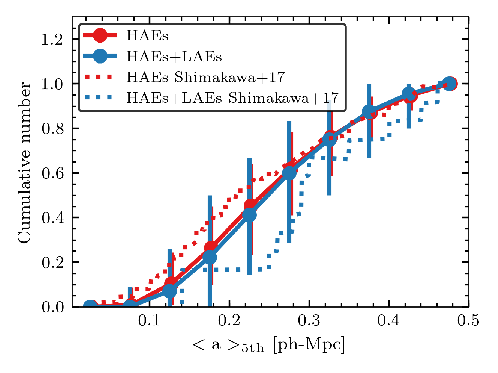
\includegraphics[width=\columnwidth]{ejemplo_figura_Hough_etal.pdf}
\caption{El tamaño de letra en el texto y en los valores numéricos de los ejes es similar al tamaño de letra de este epígrafe. Si utiliza más de un panel, explique cada uno de ellos; ej.: \emph{Panel superior:} explicación del panel superior. Figura reproducida con permiso de \cite{Hough_etal_BAAA_2020}.}
\label{Figura}
\end{figure}

\subsection{Referencias cruzadas}\label{ref}

Su artículo debe emplear referencias cruzadas utilizando la herramienta  {\sc bibtex}. Para ello elabore un archivo (como el ejemplo incluido: {\tt bibliografia.bib}) conteniendo las referencias {\sc bibtex} utilizadas en el texto. Incluya el nombre de este archivo en el comando \LaTeX{} de inclusión de bibliografía (\verb|\bibliography{bibliografia}|). 

Recuerde que la base de datos ADS contiene las entradas de {\sc bibtex}  para todos los artículos. Se puede acceder a ellas mediante el enlace ``{\em Export Citation}''.

El estilo de las referencias se aplica automáticamente a través del archivo de estilo incluido (baaa.bst). De esta manera, las referencias generadas tendrán la forma co\-rrec\-ta para un autor \citep{hubble_expansion_1929}, dos autores \citep{penzias_cmb_1965,penzias_cmb_II_1965}, tres autores \citep{navarro_NFW_1997} y muchos autores \citep{riess_SN1a_1998}, \citep{Planck_2016}.

\begin{acknowledgement}
Los agradecimientos deben agregarse usando el entorno correspondiente (\texttt{acknowledgement}).
\end{acknowledgement}

%%%%%%%%%%%%%%%%%%%%%%%%%%%%%%%%%%%%%%%%%%%%%%%%%%%%%%%%%%%%%%%%%%%%%%%%%%%%%%
%  ******************* Bibliografía / Bibliography ************************  %
%                                                                            %
%  -Ver en la sección 3 "Bibliografía" para mas información.                 %
%  -Debe usarse BIBTEX.                                                      %
%  -NO MODIFIQUE las líneas de la bibliografía, salvo el nombre del archivo  %
%   BIBTEX con la lista de citas (sin la extensión .BIB).                    %
%                                                                            %
%  -BIBTEX must be used.                                                     %
%  -Please DO NOT modify the following lines, except the name of the BIBTEX  %
%  file (whithout the .BIB extension).                                       %
%%%%%%%%%%%%%%%%%%%%%%%%%%%%%%%%%%%%%%%%%%%%%%%%%%%%%%%%%%%%%%%%%%%%%%%%%%%%%% 

\bibliographystyle{baaa}
\small
\bibliography{bibliografia}
 
\end{document}
